\chapter{Resultados}

A continuación se presentan gráficas de propiedades estructurales y termodinámicas para analizar el sistema estudiado.

% \subsubsection{Propiedades termodinámicas}

% Se muestran algunas figuras que son cálculos instantáneos de la presión y temperatura:

% \begin{figure}[!h]
%     \centering
%     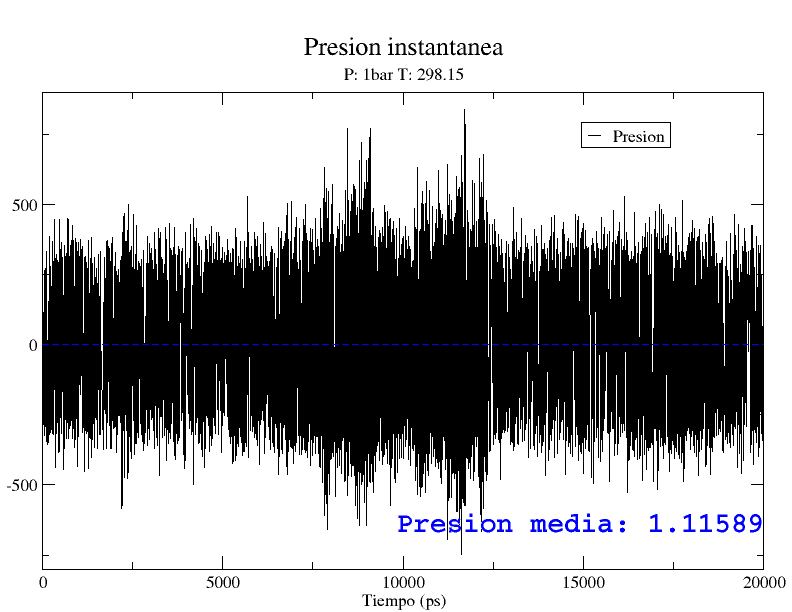
\includegraphics[width=.9\textwidth,keepaspectratio=true]{Pres298.png}
%     \caption{Gráfica de la presión instantánea del sistema a condición estandar IUPAC, la media de la presión fue 1.11589 bar}
%     \label{fig:Enertot298.15}
% \end{figure}
\section{Representación visual de la adsorción de las moléculas 2,4-D}

La figura \ref{fig:Conffinal370} es una representación visual de la adsorción de las moléculas 2,4-D en el nanotubo. Esta adsorción que se observa en la representación visual, se replica en todas las configuraciones finales del sistema en todas las temperaturas simuladas.

\begin{figure}[!h]
    \centering
    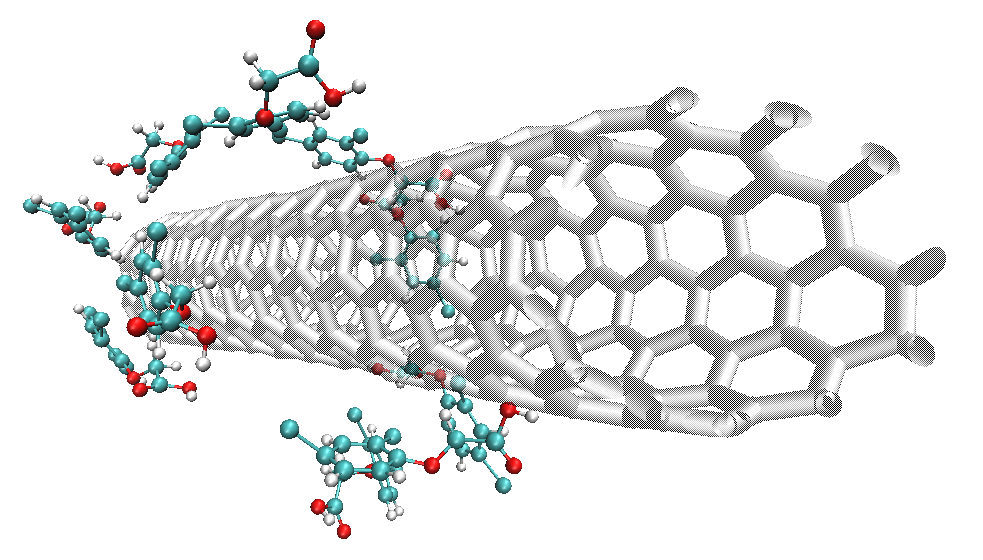
\includegraphics[width=0.6\textwidth,keepaspectratio=true]{resultados/all-new-370K.png}
    \caption{Nanotubo y moléculas de 2,4-D en la configuración final a 370 K.}
    \label{fig:Conffinal370}
\end{figure}

\section{Función de distribución radial}

Las funciones de distribución radial fueron calculado en un rango de 280 a 370. En el caso de pares átomo-átomo se calcularon los pares entre átomos de oxígeno-oxígeno, oxígeno-hidrógeno y hidrógeno-hidrógeno del agua, también los pares entre carbono del nanotubo de carbono y ácido 2,4-diclorofenoxiacético que son carbono-oxígeno de 2,4-D, carbono-hidrógeno de 2,4-D, carbono-cloro de 2,4-D y carbono-carbono de 2,4-D. Igualmente se calcularon los pares entre centro de masa del nanotubo y átomo de 2,4-D los cuales son centro de masa del nanotubo-oxígeno, centro de masa del nanotubo-hidrógeno, centro de masa del nanotubo-cloro y centro de masa del nanotubo-carbono. Además se calcularon la funciones para los pares centro de masa del nanotubo de carbono-centro de masa de la molécula 2,4-D y carbono del nanotubo-centro de masa de 2,4-D.\\

% \begin{itemize}
%     \item átomo A - átomo B:
%         \begin{itemize}
%             \item agua-agua: OW-OW, OW-HW, HW-HW
%         \end{itemize}
%         % \begin{itemize}
%         %     \item agua-2,4-D: OW-OD, OW-ClD, OW-HD, HW-HD, HW-ClD
%         % \end{itemize}
%         % \begin{itemize}
%         %     \item agua-CNT(6,5): OW-C,  HW-C
%         % \end{itemize}
%         \begin{itemize}
%             \item 2,4-D-CNT(6,5): OD-C, HD-C, ClD-C, CD-C
%         \end{itemize}
%         % \begin{itemize}
%         %     \item 2,4-D-2,4-D: OD-OD, HD-HD, ClD-ClD, CD-CD, ClD-HD, OD-HD
%         % \end{itemize}
%         % \begin{itemize}
%         %     \item CNT(6,5)-CNT(6,5): C-C
%         % \end{itemize}
%     \item centro de masa A - centro de masa B:
%         \begin{itemize}
%             \item 2,4-D-CNT(6,5): centro de masa CNT - centro de masa 2,4-D, centro de masa de ambas tapas CNT - centro de masa 2,4-D
%         \end{itemize}
%     \item centro de masa A - átomo B:
%         \begin{itemize}
%             \item CNT(6,5)-2,4-D: centro de masa CNT - ClD, centro de masa CNT - HD, centro de masa CNT - OD, centro de masa CNT - Cl1D
%         \end{itemize}
%         % \begin{itemize}
%         %     \item agua-2,4-D: OW-OD, OW-ClD, OW-HD, HW-HD, HW-ClD
%         % \end{itemize}
% \end{itemize}

% A continuación se presentan algunas gráficas y figuras significativas para posteriormente para analizar.\\

% \newpage

\begin{figure}[!hbt]
    \centering
    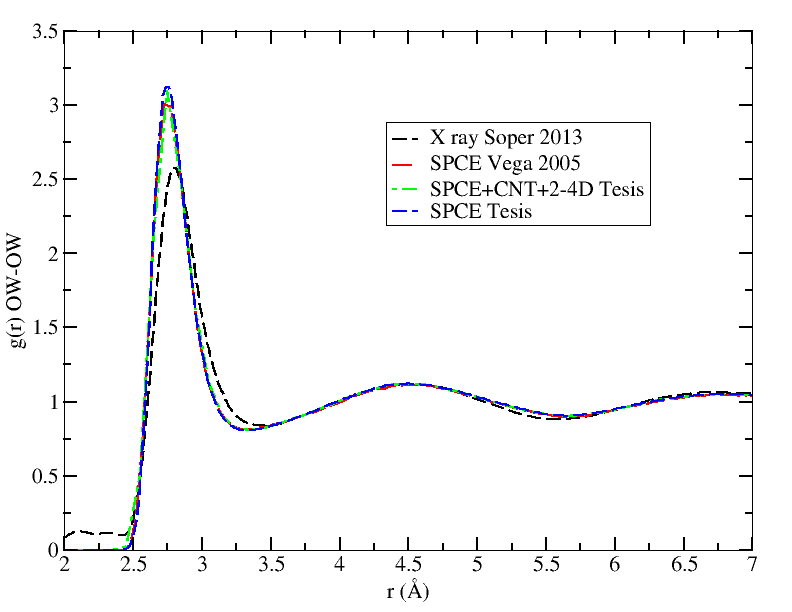
\includegraphics[width=0.7\textwidth,keepaspectratio=true]{resultados/gOOcartel.png}
    \caption{Función de distribución radial O-O de agua a 1 bar: comparación entre resultados experimentales (Soper, 2013)4, simulación de agua SPCE a 300 K (Vega, 2005)3, nuestra simulación de agua SPCE a 298.15 K, y función calculada en la mezcla de agua/herbicida a 298.15 K.}
    \label{fig:OO}
\end{figure}

En la figura \ref{fig:OO} se presenta una comparación de la función distribución radial del par oxigeno-oxigeno de agua: la linea negra corresponde a la función experimental obtenida por Soper \cite{Soper2013} a 298 K, las lineas de color roja y azul corresponden a funciones obtenidas en simulacion de agua pura de Vega \cite{vega2005} a 300 K y de nosotros a 298.15 K, respectivamente; la linea verde corresponde a la funcion obtenida en la mezcla presentada en este trabajo. Observamos un acuerdo entre funciones de distribución radial de simulación, igualmente la diferencia en la función obtenida por Soper en comparación con las otras era lo esperado. Por lo tanto, el agua sigue manteniendo la misma estructura ya sea en simulaciones de agua pura o en la mezcla de este trabajo.\\
% En la figura \ref{fig:24D_CNT_298_15_atom_atom} comparamos diferentes funciones de distribución radial a 298.25 K que se caracterizan como: carbono del nanotubo - átomo de 2,4-D. La función Cl(2,4-D)-C(CNT) y C(2,4-D)-C(CNT) tienen una distribución similar con dos máximos en aproximadamente $4.3<r1<4.5$ y $10.8<r2<11$ angstroms(\AA); y los pares  H(2,4-D)-C(CNT) y O(2,4-D)-C(CNT) tienen similares máximos con dos máximos en $r=5$ y $r=10.62$ \AA. Además, se puede observar que el hidrógeno de 2,4-D se encuentra mas cercano al carbón del nanotubo en $r\sim 2.3$\AA y el mas probable de los átomos en ser encontrado es el carbono de 2,4-D dado otro carbono en $r\sim 4.5$. \\

\newpage

\begin{figure}[!hbt]
    \centering
    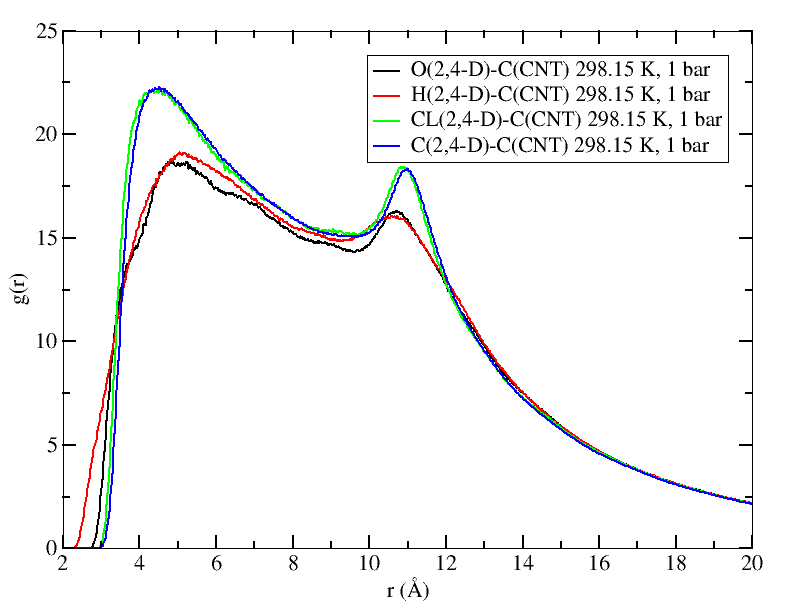
\includegraphics[width=0.6\textwidth,keepaspectratio=true]{resultados/gr_24D_CNT_298_15_atom_atom.png}
    \caption{Funciones de distribución radial átomo-átomo entre el C del nanotubo y átomos O, H, CL y C del 2,4-D a 298.15 K y 1 bar.}
    \label{fig:24D_CNT_298_15_atom_atom}
\end{figure}

En la figura \ref{fig:24D_CNT_298_15_atom_atom} se compararon diferentes funciones de distribución radial a 298.25 K del tipo átomo-átomo. La curva azul y verde corresponden a las funciones carbono del nanotubo-carbono de 2,4-D y carbono del nanotubo-cloro de 2,4-D respectivamente, entre estas funciones observamos que son similares con dos máximos en la distribución, $\sim 4.3$ \AA\  y $\sim 11$ \AA. La curva roja corresponde al par carbono del nanotubo-hidrógeno de 2,4-D, esta función comienza en $\sim 2$ \AA\  y el primer máximo se encuentra en $\sim 5$ \AA; y la curva negra corresponde a la función carbono del nanotubo-oxígeno de 2,4-D con un máximo alrededor de $\sim 5$ \AA. Observamos que la mayor concentración de moléculas alrededor del nanotubo esta entre el rango de $\sim 4.3$ \AA\  y $\sim 5$ \AA, donde el hidrógeno de 2,4-D es el mas cercano al nanotubo como las gráficas lo indican.

\newpage

\section{Número de coordinación}

\begin{figure}[!ht]
\begin{subfigure}{.5\textwidth}
  \centering
  % include first image
  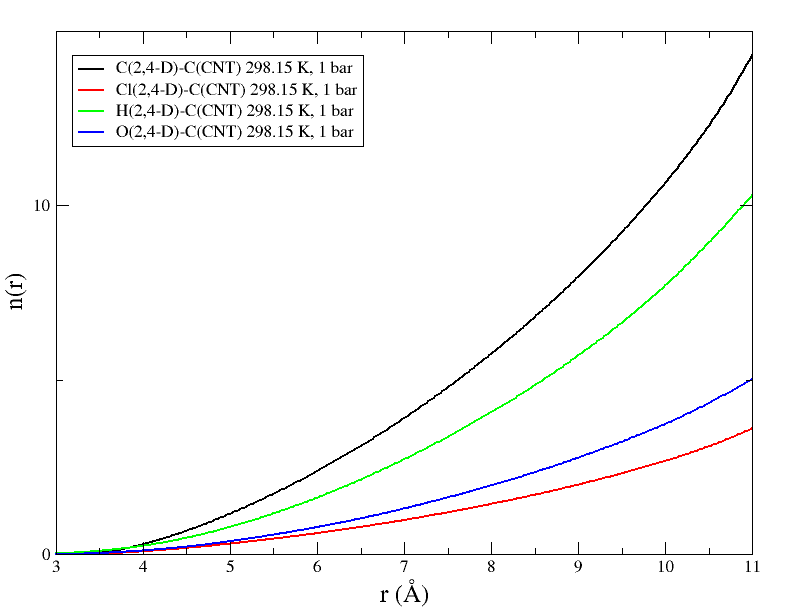
\includegraphics[width=1\linewidth]{resultados/gr_24D_CNT_298_15_atom_atom_cn_alt.png}  
  \caption{Número de coordinación de la figura \ref{fig:24D_CNT_298_15_atom_atom}.}
  \label{fig:24D_CNT_298_15_atom_atom_cn}
\end{subfigure}
\begin{subfigure}{.5\textwidth}
  \centering
  % include second image
  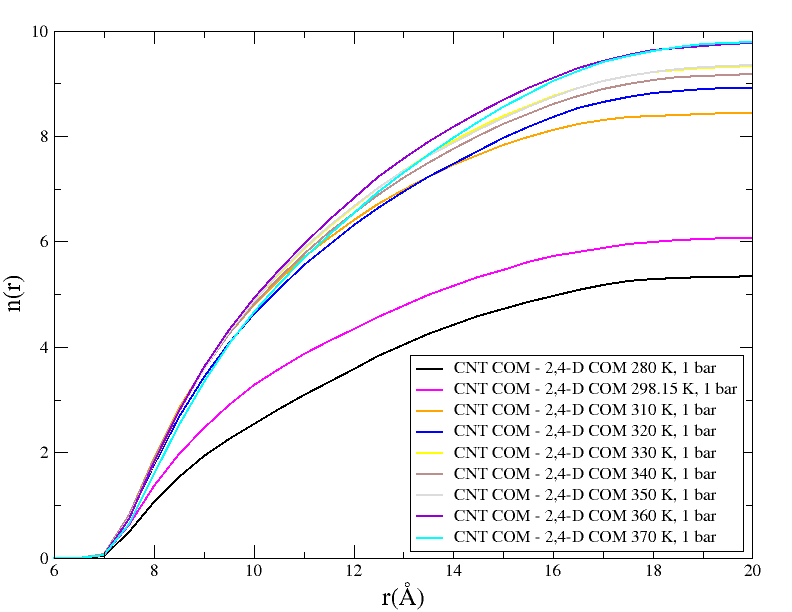
\includegraphics[width=1\linewidth]{resultados/cmnt_cmd_alltemp.png}  
  \caption{Número de coordinación de la función de distribución radial de centros de masa del nanotubo y 2,4-D en el rango de temperaturas 280-370 K.}
  \label{fig:24D_CNT_alltemp_CM-CM_cn}
\end{subfigure}
\caption{Números de coordinación}
\label{fig:24D_CNT_298_15_alltemp_atom_atom_cn}
\end{figure}

La figura \ref{fig:24D_CNT_298_15_atom_atom_cn} es el número de coordinación de la figura \ref{fig:24D_CNT_298_15_atom_atom}, se observa que a la distancia $\sim 5$ \AA\ hay $\sim 1$ átomo de hidrógeno y de carbono en promedio. En el caso de figura \ref{fig:24D_CNT_alltemp_CM-CM_cn} hay dos observaciones importantes, el número de moléculas alrededor del centro de masa del nanotubo aumentan con la temperatura y a 12 \AA\  del centro de masa del nanotubo se encuentran de 3 a 7 moléculas 2,4-D según la temperatura a la que se encuentra el sistema. En las figuras \ref{fig:24DCOM} y \ref{fig:CNTCOM} se observan los centros de masa de la molécula 2,4-D y el nanotubo de carbono respectivamente.\\

\begin{figure}[!h]
    \centering
    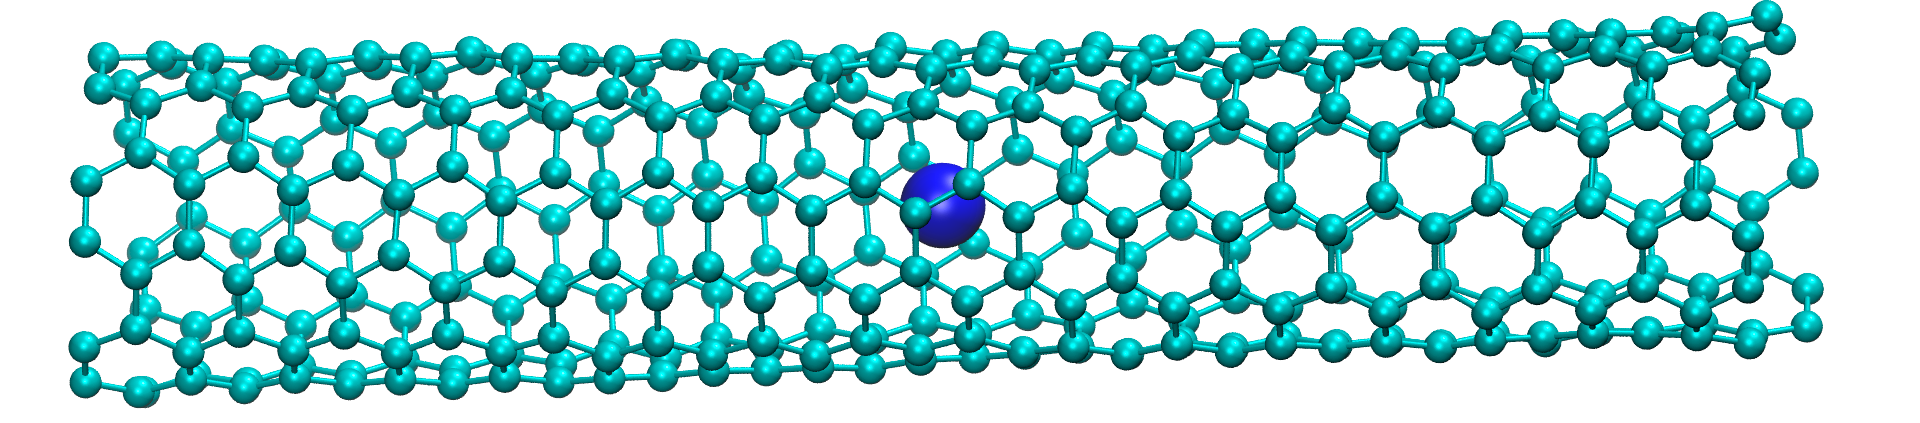
\includegraphics[width=.9\textwidth,keepaspectratio=true]{resultados/CNTCOM.png}
    \caption{Centro de masa del nanotubo de carbono (6,5),  presentado en este trabajo y representado por la esfera azul.}
    \label{fig:CNTCOM}
\end{figure}

\begin{figure}[!h]
    \centering
    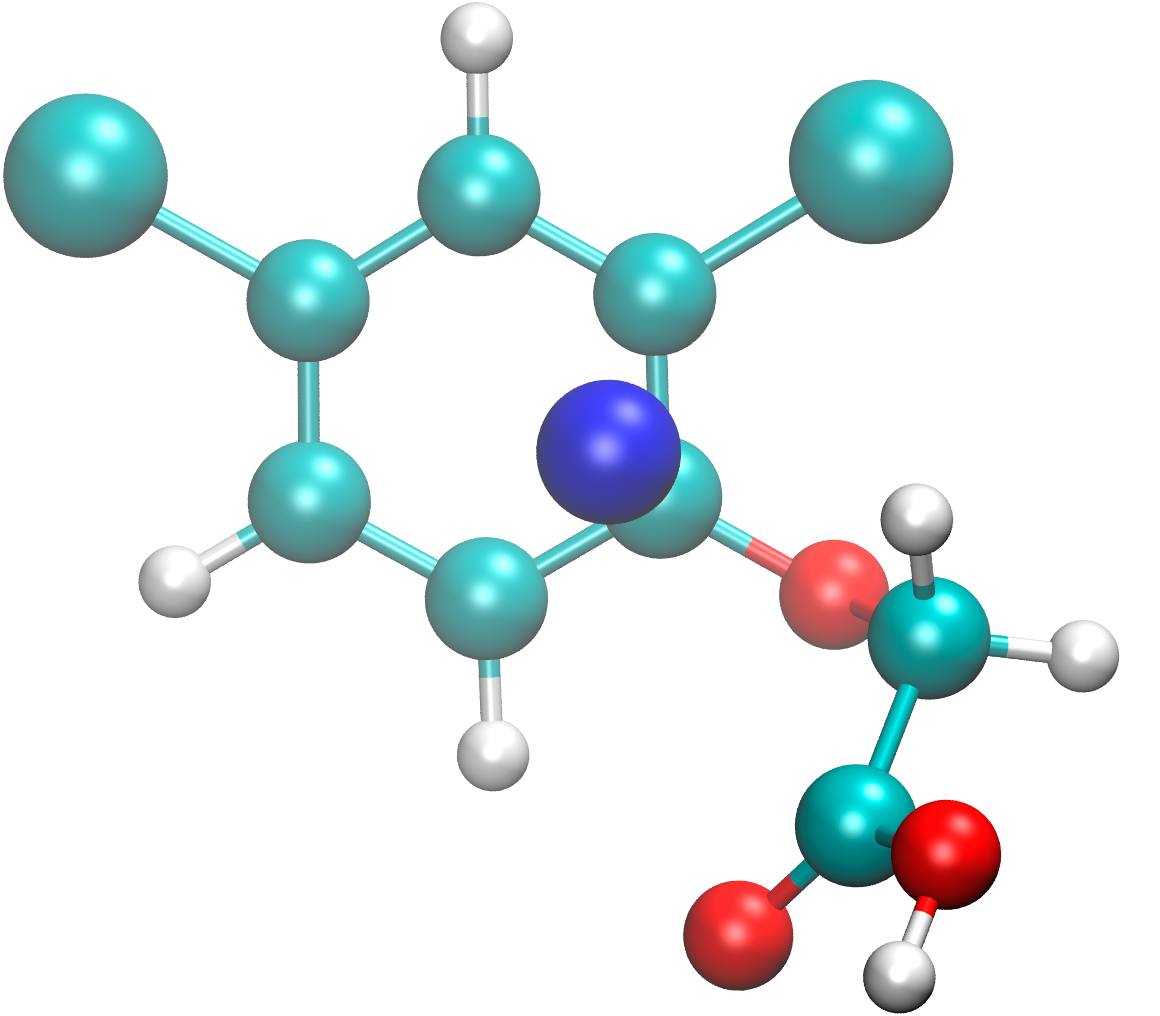
\includegraphics[width=.5\textwidth,keepaspectratio=true]{resultados/24DCOM.png}
    \caption{Centro de masa de la molécula de 2,4-D,  presentado en este trabajo y representado por la esfera azul.}
    \label{fig:24DCOM}
\end{figure}

Todas las funciones indican una cercanía y un interacción adsorbente entre el nanotubo de carbono y la molécula del herbicida. Esto se observa en todos los sistemas visualmente, por ejemplo, en la figura \ref{fig:Conffinal370}. 

% -------------------------------------------------------------------
% Funciones g(r)  [átomo A - átomo B]
% -------------------------------------------------------------------
% agua-agua:  g_OO,  g_OH,  g_HH   en funcion de la T (275 - 370 K) 
% agua-42D:   g_(OW-OD), g_(HW-HD), g_(OW-ClD), g_(HW-ClD), g_(OW-HD)
% agua-CNT:  g_(OW-C),  g_(HW-C)

% 42D-CNT:  g_(OD-C),  g_(HD-C),  g_(ClD-C),  g_(CD-C)
% 42D-42D:   g_(OD-OD),  g_(HD-HD),  g_(ClD-ClD),  g_(CD-CD),  g_(ClD-HD),  g_(OD-HD)

% CNT-CNT:   g_(C-C)
% ------------------------------------------------------------------------
% Funciones g(r)  [cm M - cm N]
% ------------------------------------------------------------------------
% CNT-42D:   g_(cm CNT - cm D),  g_(cm tapa CNT - cm D)

% ------------------------------------------------------------------------ 
% Funciones g(r)  [cm M -  átomo B]
% ------------------------------------------------------------------------
% CNT-42D:  g_(cm NT - ClD),  g_(cm NT - HD),  g_(cm NT - OD),  g_(cm NT - Cl1D), g_(cm NT - OD)
% CNT-agua:  g_(cm NT - OW),  g_(cm NT - HW)

